\documentclass[12pt]{article}
\usepackage{graphicx}%Package um Grafiken einzufügen
\graphicspath{ {assets/} }
\usepackage[ngerman]{babel}%Sprache Deutsch einstellen
\usepackage[headheight=15pt, a4paper, left=40mm, top=20mm, bottom=20mm, right=20mm]{geometry}
%\usepackage[]{fontspec}
%\setmainfont{Inter.ttf}
\usepackage[]{fancyhdr}
\pagestyle{fancy}
%\setlength{\headheight}{16pt}
\lhead{\leftmark}
\rhead{Phillip Bronzel} 

\usepackage[style=authoryear, backend=biber]{biblatex}
\addbibresource{references.bib}
\usepackage{csquotes}

\title{Machine Learning in Smartphone Apps}
\date{Phillip Bronzel \today}
\author{ASGSG Informatik, 2020/2021}

\begin{document}
  \maketitle
  \pagenumbering{gobble}
  \begin{center}
   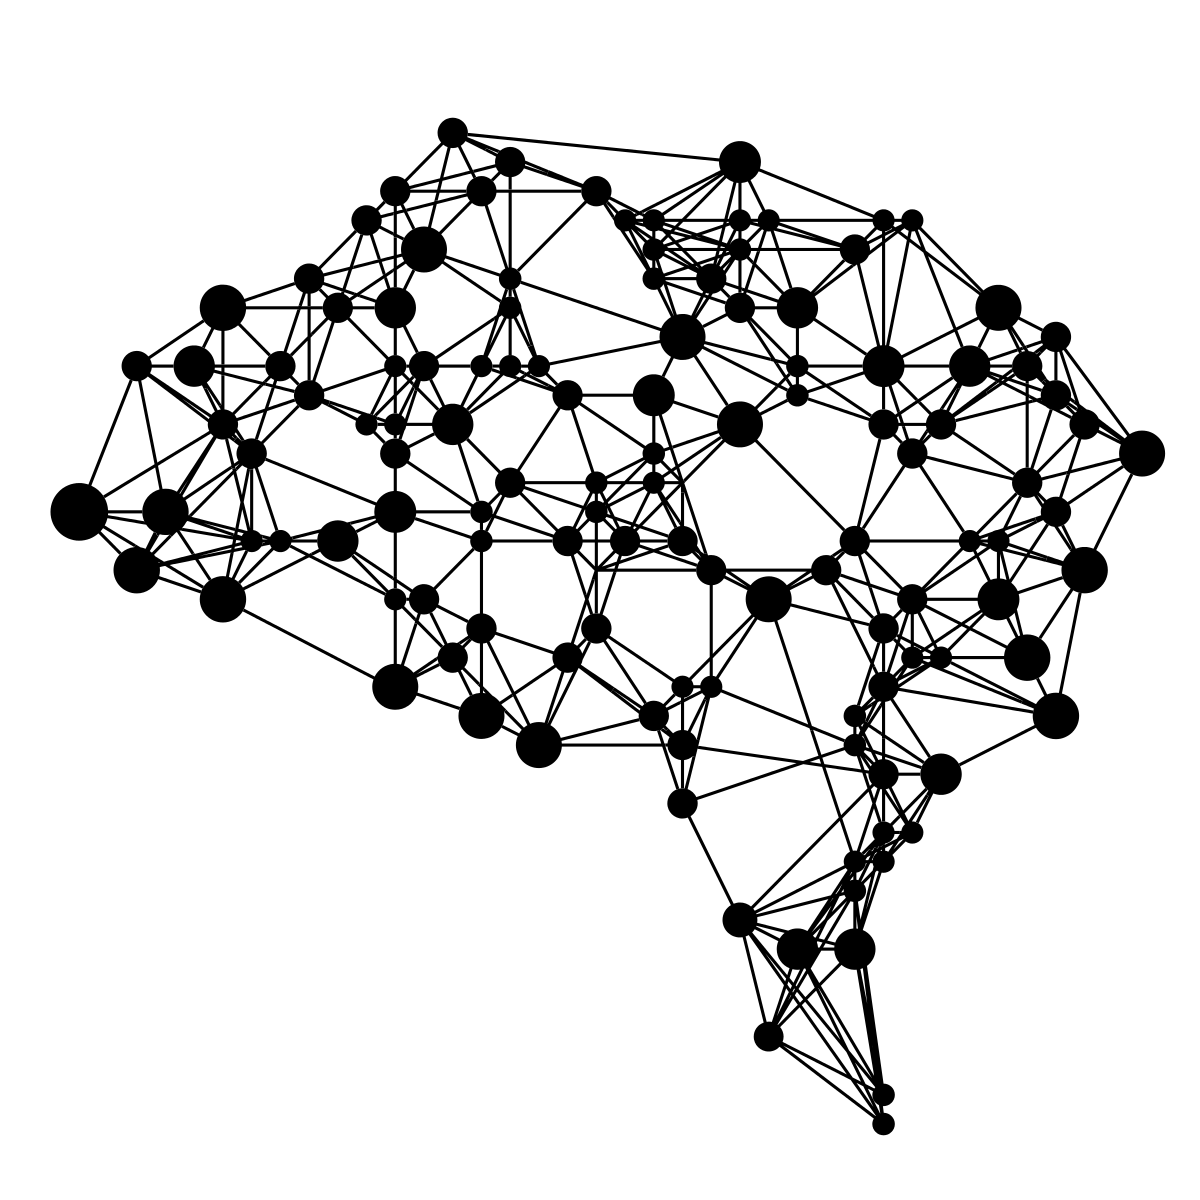
\includegraphics[totalheight=10cm]{titlepage.png}
   \cite{titlepageimage}
  \end{center}

  \newpage
  \vspace*{\fill}
  \input{lib/erklärung.tex}
  \vspace*{\fill}

  \newpage
  \pagenumbering{arabic}
  \tableofcontents

  \newpage
  \section{Einführung}
  \input{lib/einführung.tex}%TODO: Kapitel der App einfügen

  \newpage
  \printbibliography[heading=bibintoc, title={Literaturverzeichnis}]
\end{document}